
\chapter{Sharing the CPU}

This chapter introduces the mechanisms by which an operating system (OS) manages access to the CPU, ensuring both security and fairness among processes. We discuss CPU privilege levels, the limited direct execution model, and the role of system calls (syscalls) in process management.
\vfill
\section{CPU Privilege Level}

\textbf{Professor Analogy -} Imagine you have children who want to watch TV. You can either keep the remote with you and ask them to call you whenever they need to change the channel, or you can enable Kids Mode on the TV, allowing them limited access without needing to ask for permission each time. \\
The CPU operates in different modes to regulate access to its instruction set:
\begin{itemize}
  \item[-] \textbf{Low Privilege (User Mode):} A normal process or thread runs in this mode and can execute only a restricted subset of instructions.
  \item[-] \textbf{High Privilege (Kernel Mode):} The operating system runs in this mode and has full access to all instructions and hardware resources.
\end{itemize}

When a regular thread executes, the CPU remains in low privilege mode. Conversely, OS code runs in high privilege mode, allowing it to perform otherwise restricted operations. This design follows the principle of least privilege, ensuring that processes have only the necessary level of access.

\begin{center}
  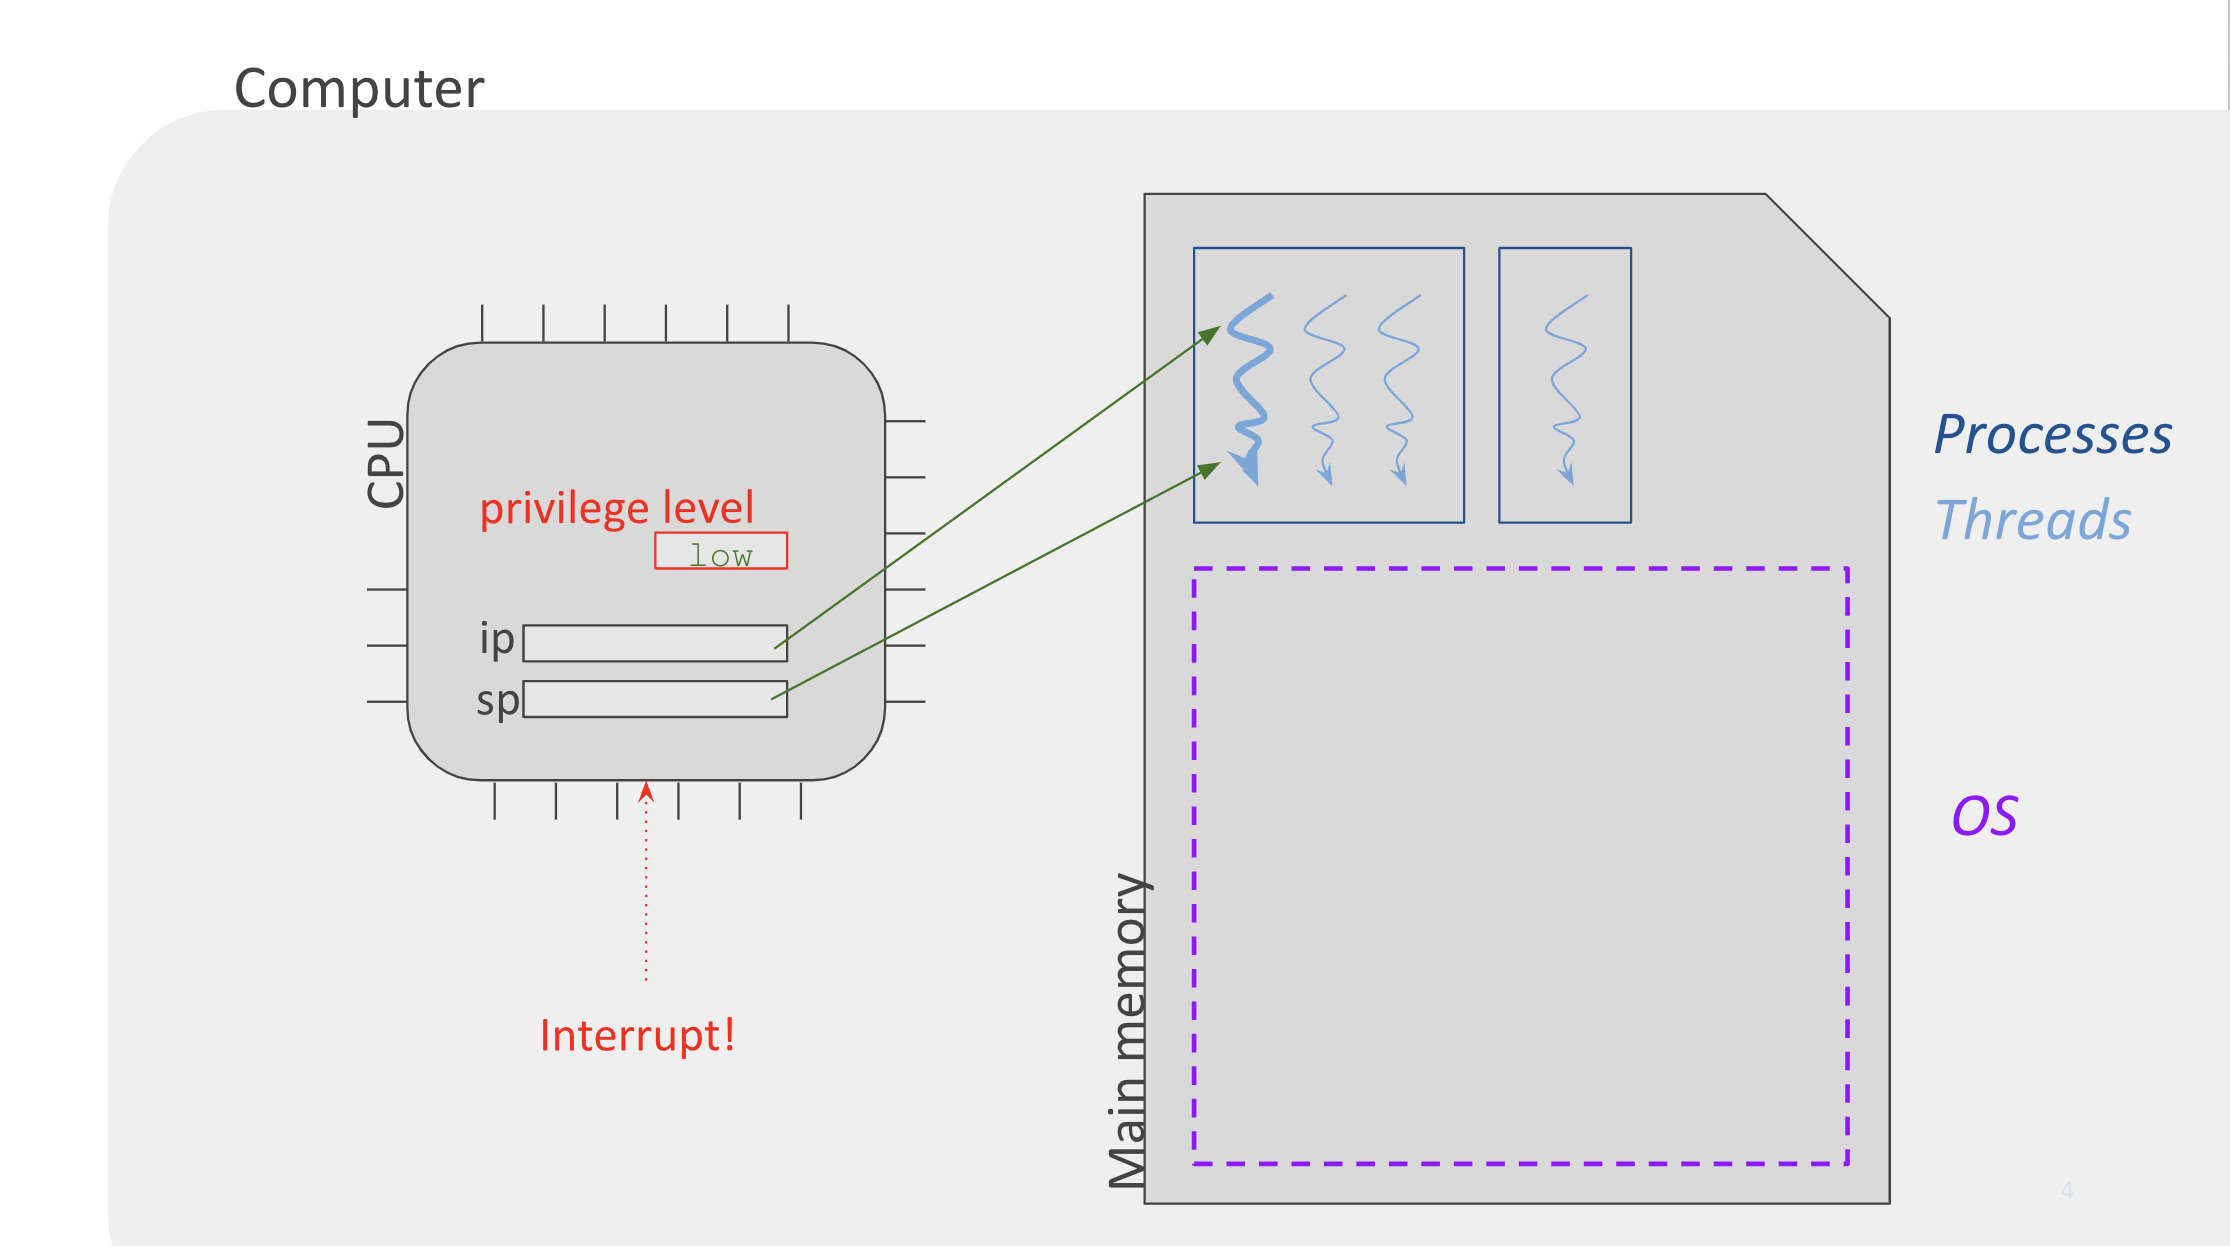
\includegraphics[width=0.8\textwidth]{chapters/L3/images/priviledge.png}
\end{center}
\newpage
\subsection{Limited Direct Execution}
\textbf{Professor Analogy cont. -} The children have direct access to the TV but are restricted by Kids Mode. \\
Limited direct execution is a method that allows a thread to run directly on the CPU while enforcing certain restrictions:
\begin{itemize}
  \item[-] \emph{Direct Execution:} The CPU executes the thread's instructions without any intermediate emulation.
  \item[-] \emph{Limited:} The thread cannot perform operations that require high privileges; instead, it must request system assistance via syscalls.
\end{itemize}

This approach minimizes overhead while ensuring that potentially unsafe operations are controlled by the OS.
\section{The OS as a Special Program}
The operating system (OS) is a fundamental software layer that manages hardware resources and provides essential services for user applications. Unlike typical applications, the OS operates at different privilege levels and ensures secure and efficient execution of processes and threads.

\subsection{CPU Privilege Levels and Execution Modes}

The OS shares the CPU and main memory with normal user processes and threads. However, its execution mode differs based on its role at any given time:

\begin{itemize}
  \item[-] When the OS executes, the CPU may be in \textbf{high privilege mode} (kernel mode), allowing it unrestricted access to all system resources.
\item[-] When a normal process or thread executes, the CPU is in \textbf{low privilege mode} (user mode), restricting access to critical system resources.
\end{itemize}

This privilege system exists primarily for security reasons, enforcing the \textbf{principle of least privilege}, where each process has only the necessary access rights required to perform its task. 

\subsection{The Kernel: Core Component of the OS}

A key component of the OS is the \textbf{kernel}, responsible for:

\begin{itemize}
  \item[-] Creating and managing processes and threads.
  \item[-] Allocating system resources (CPU time, memory, I/O devices, etc.).
  \item[-] Ensuring that each process has a designated portion of memory, including stack, data, and text segments.
  \item[-] Enforcing security and isolation between processes.
\end{itemize}

The kernel always runs in \textbf{high privilege mode} (kernel mode), which is why this mode is sometimes referred to as \textit{kernel mode}. 

\subsection{Process Management and Context Switching}

The OS does not execute continuously but rather runs only when necessary. It performs essential tasks, prepares the environment for the next process, and then switches out, allowing user processes to execute.

\begin{itemize}
  \item[-] The OS uses \textbf{context switching} to transition between processes efficiently, preserving the state of the current process before switching to another.
  \item[-] By switching between kernel mode and user mode, the OS ensures that user applications run securely and do not directly manipulate hardware resources.
\end{itemize}

\subsection*{The Loader: Setting Up Process Memory}

Another critical component of the OS is the \textbf{loader}, which is responsible for preparing a program for execution: \\
\begin{minipage}{0.45\textwidth}
\begin{itemize}
    \item[-] The loader completes the setup of the process's memory image.
    \item[-] It copies the command-line arguments used to launch the program (e.g., \texttt{ls -a}, where \texttt{-a} is an argument).
    \item[-] These arguments are stored in the \textbf{stack} of the main thread of the new process to ensure accessibility.
\end{itemize}
\end{minipage} \hfill \vline \hfill 
\begin{minipage}{0.45\textwidth}
If these arguments were stored in the loader's stack instead, the process would not be able to access them after execution begins.
\begin{center}
    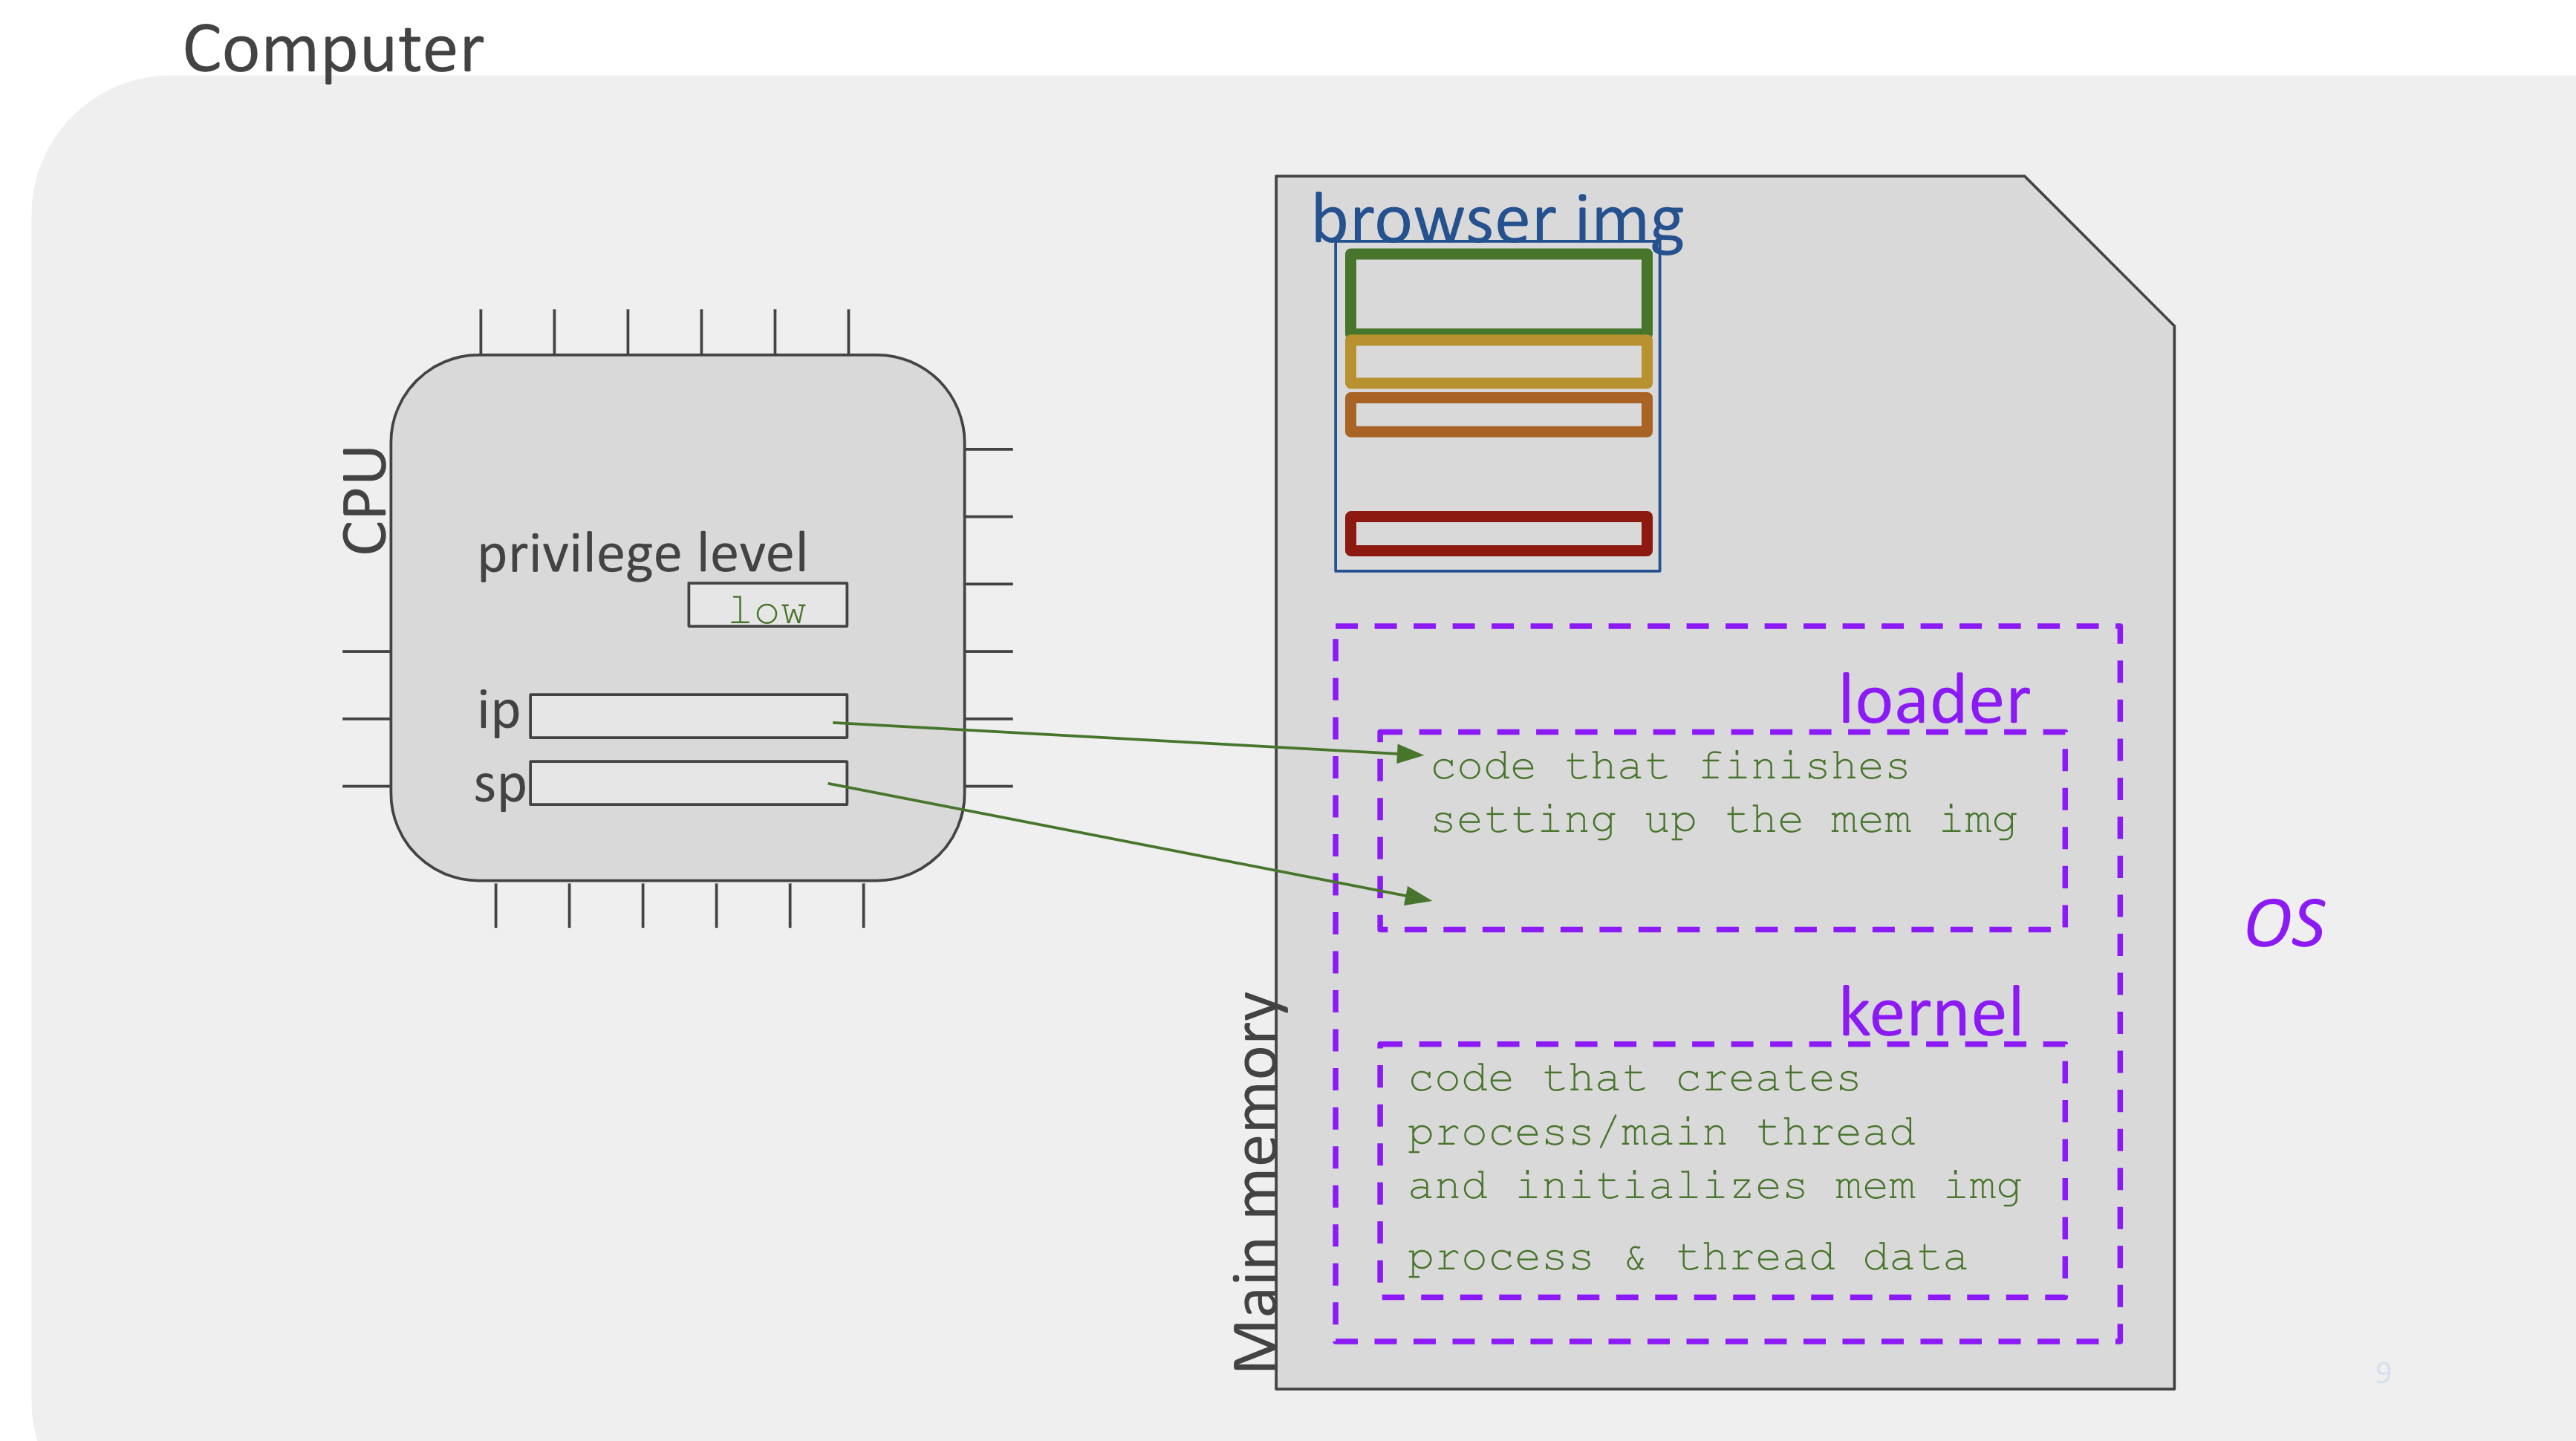
\includegraphics[width=1.1\textwidth]{chapters/L3/images/kernel.png}
\end{center}
\end{minipage} \\[10px]

This layered privilege model ensures a secure and efficient execution environment, maintaining stability and protection across all processes within the system.
\subsection{Syscalls}
\textit{Personal Remark - Syscalls are NOT needed when executing OS code, they only allow to cross the priviledged barrier when running a unpriviledged code.}
A \emph{syscall} is the mechanism by which a user process requests services from the OS. When a syscall is invoked:
\begin{enumerate}
  \item The CPU temporarily elevates the privilege level.
  \item The control is transferred to the OS to execute the privileged code.
  \item If the syscall involves an I/O operation, the process may be blocked while waiting for a response, and the CPU may perform a context switch to another thread.
  \item Once the operation is complete, the CPU returns to low privilege.
\end{enumerate}

\begin{center}
  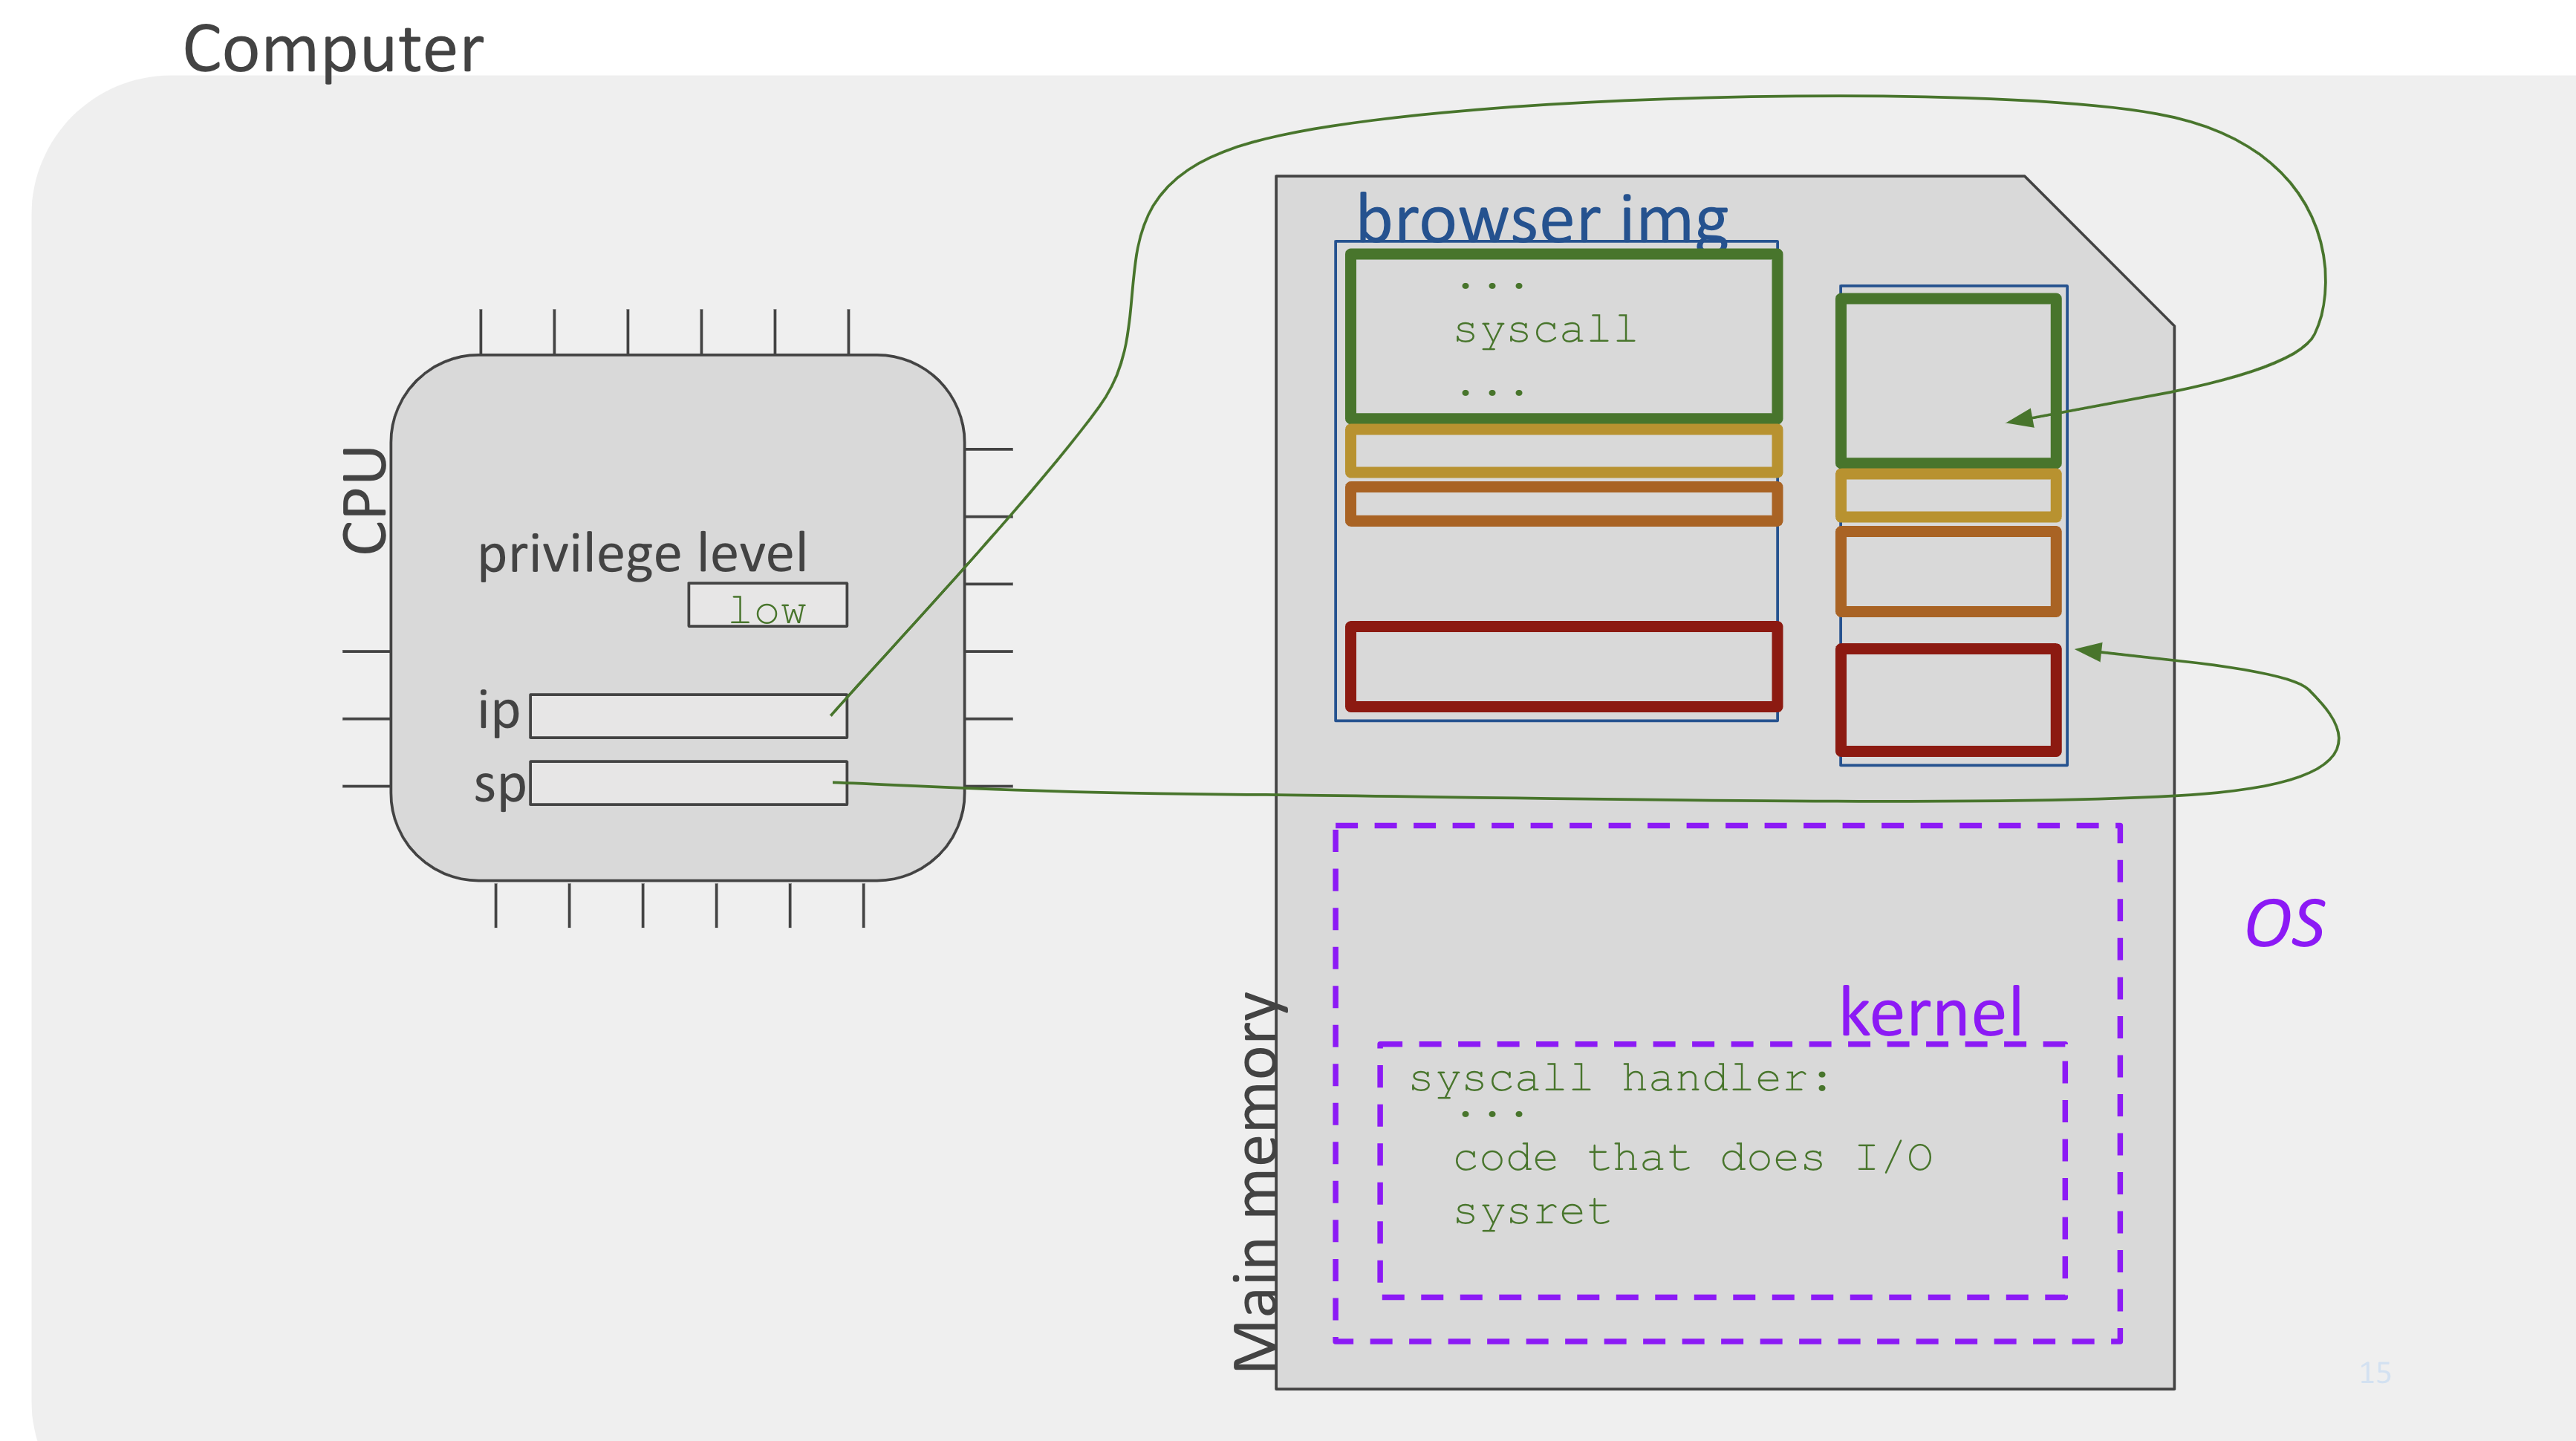
\includegraphics[width=0.8\textwidth]{chapters/L3/images/parallel-syscall.png}
\end{center}
\newpage
\subsection{Process I/O and Scheduling}
When a process initiates an I/O operation:\\
\begin{minipage}[htp]{0.45\textwidth}
\begin{itemize}
  \item It transitions from \emph{Running} to \emph{Blocked} as it waits for the I/O to complete.
  \item Once the I/O is complete, the process moves to the \emph{Ready} state.
  \item The OS scheduler then selects processes from the Ready queue to run, ensuring fair CPU utilization.
\end{itemize}
\end{minipage} 
\hfill 
\vline 
\hfill 
\begin{minipage}[htp]{0.45\textwidth}
\begin{center}
  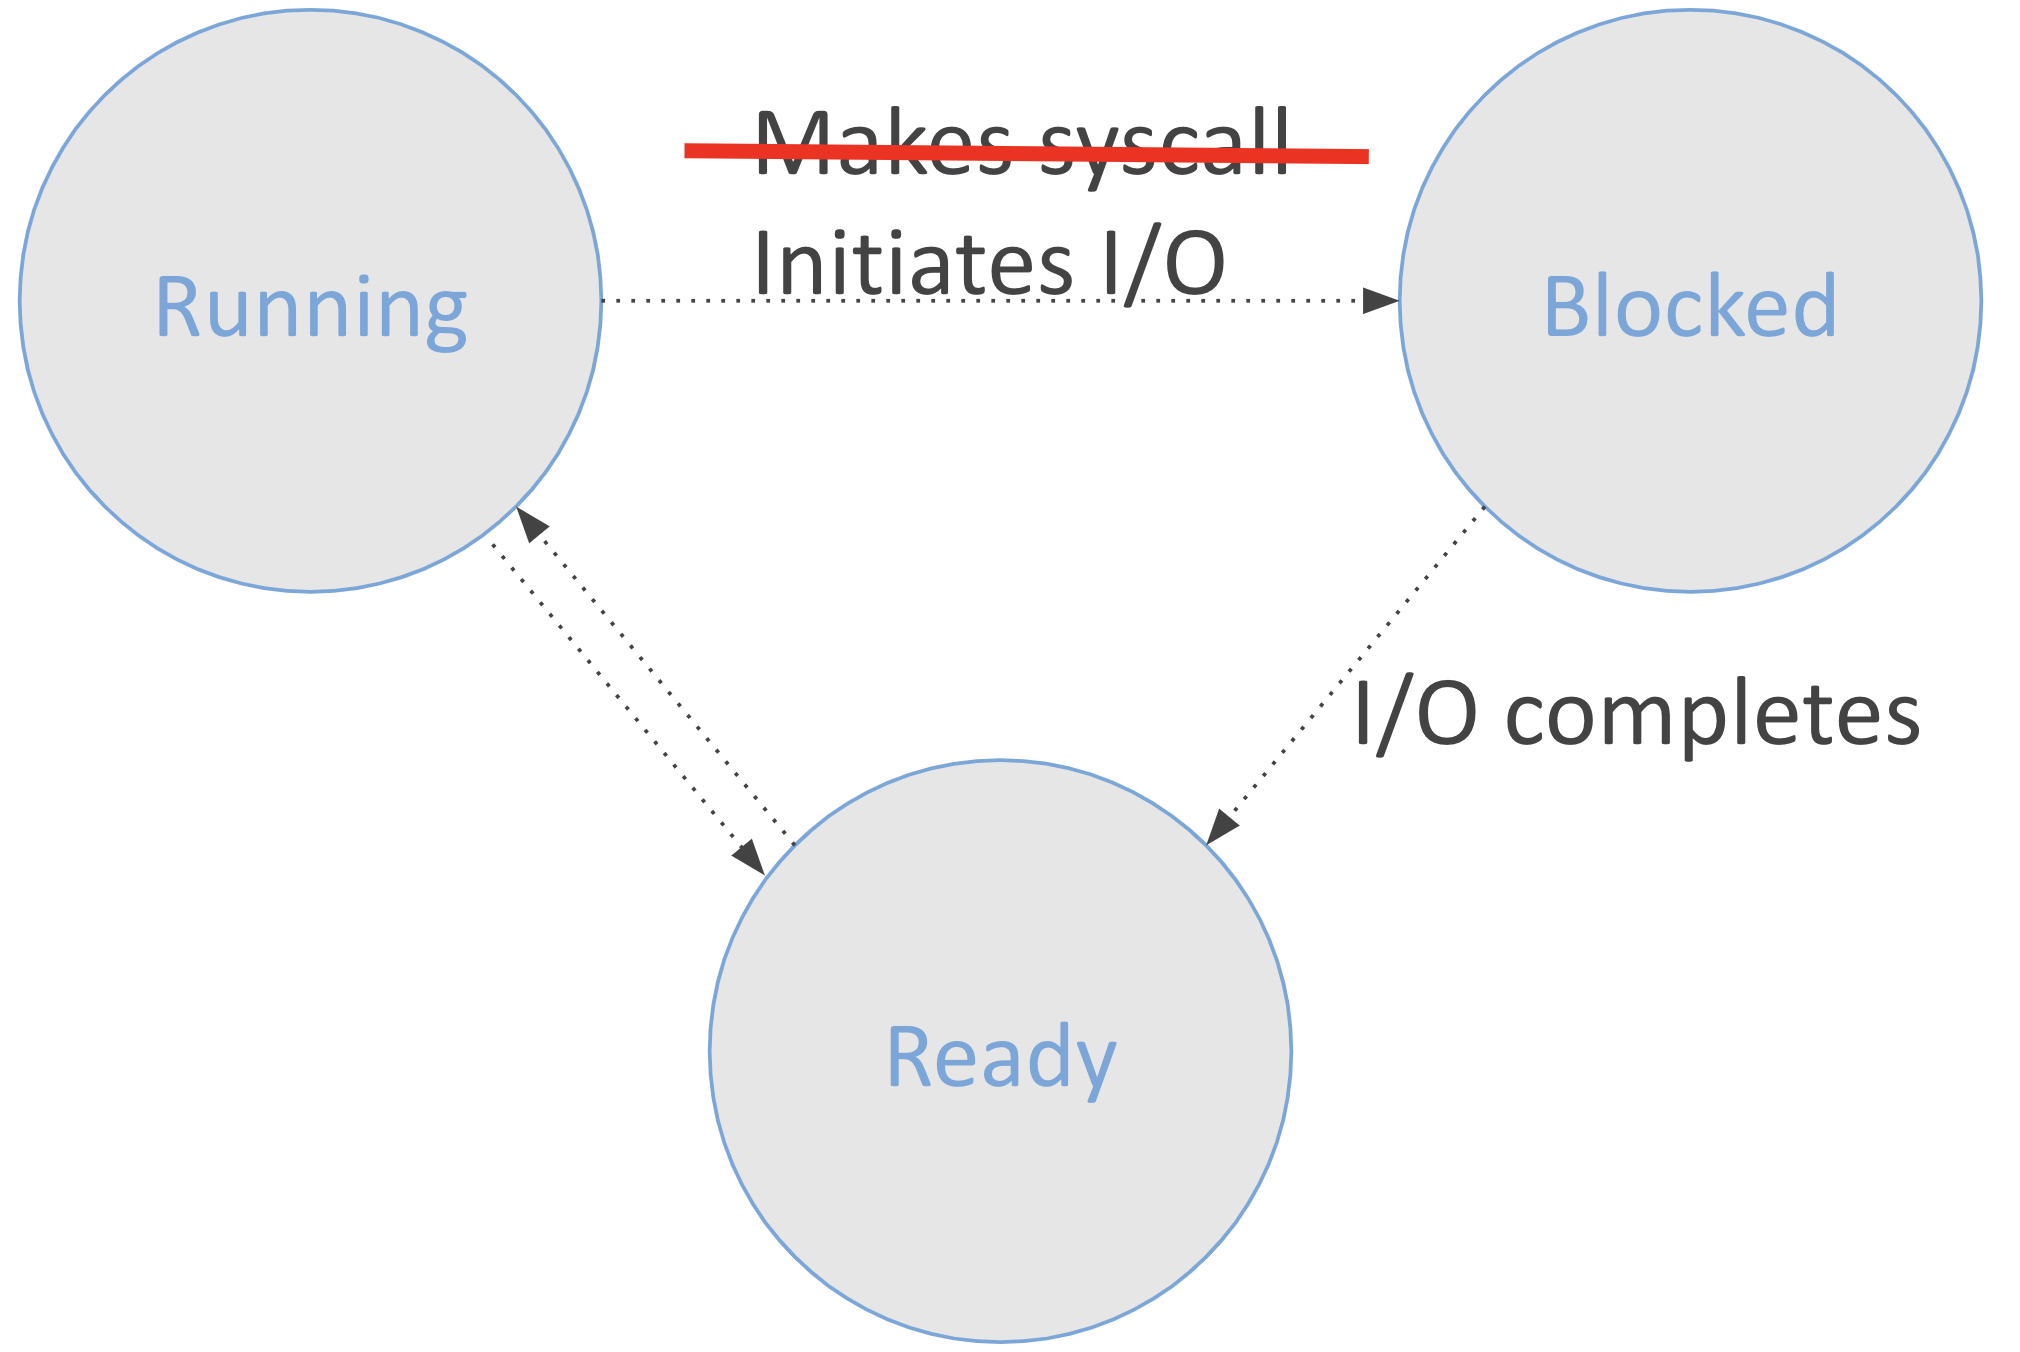
\includegraphics[width=0.95\textwidth]{chapters/L3/images/diagram.png}
\end{center}
\end{minipage}
\vspace{20px}
\section{The Kernel's Job cont.}
The Kernel handles several types of events:
\begin{itemize}[topsep=3px]
  \item[-] \textbf{Syscalls:} Requests from running threads for system-level services.
  \item[-] \textbf{Exceptions/Traps:} Synchronous signals generated when a thread executes an illegal or erroneous operation (e.g., division by zero).
  \item[-] \textbf{Interrupts:} Asynchronous signals from external devices (e.g., mouse events, network packets) requiring immediate attention.
\end{itemize}
\vspace{10px}
\begin{minipage}[htp]{0.45\textwidth}
\subsubsection*{Exception Handling}
\textit{What happens if the browser executes unauthorized code or encounters an error, such as dividing by zero ?}\\
When a process executes an illegal operation, the CPU raises an exception. The kernel then takes over to handle the error safely.
\vspace{8px}
\begin{center}
  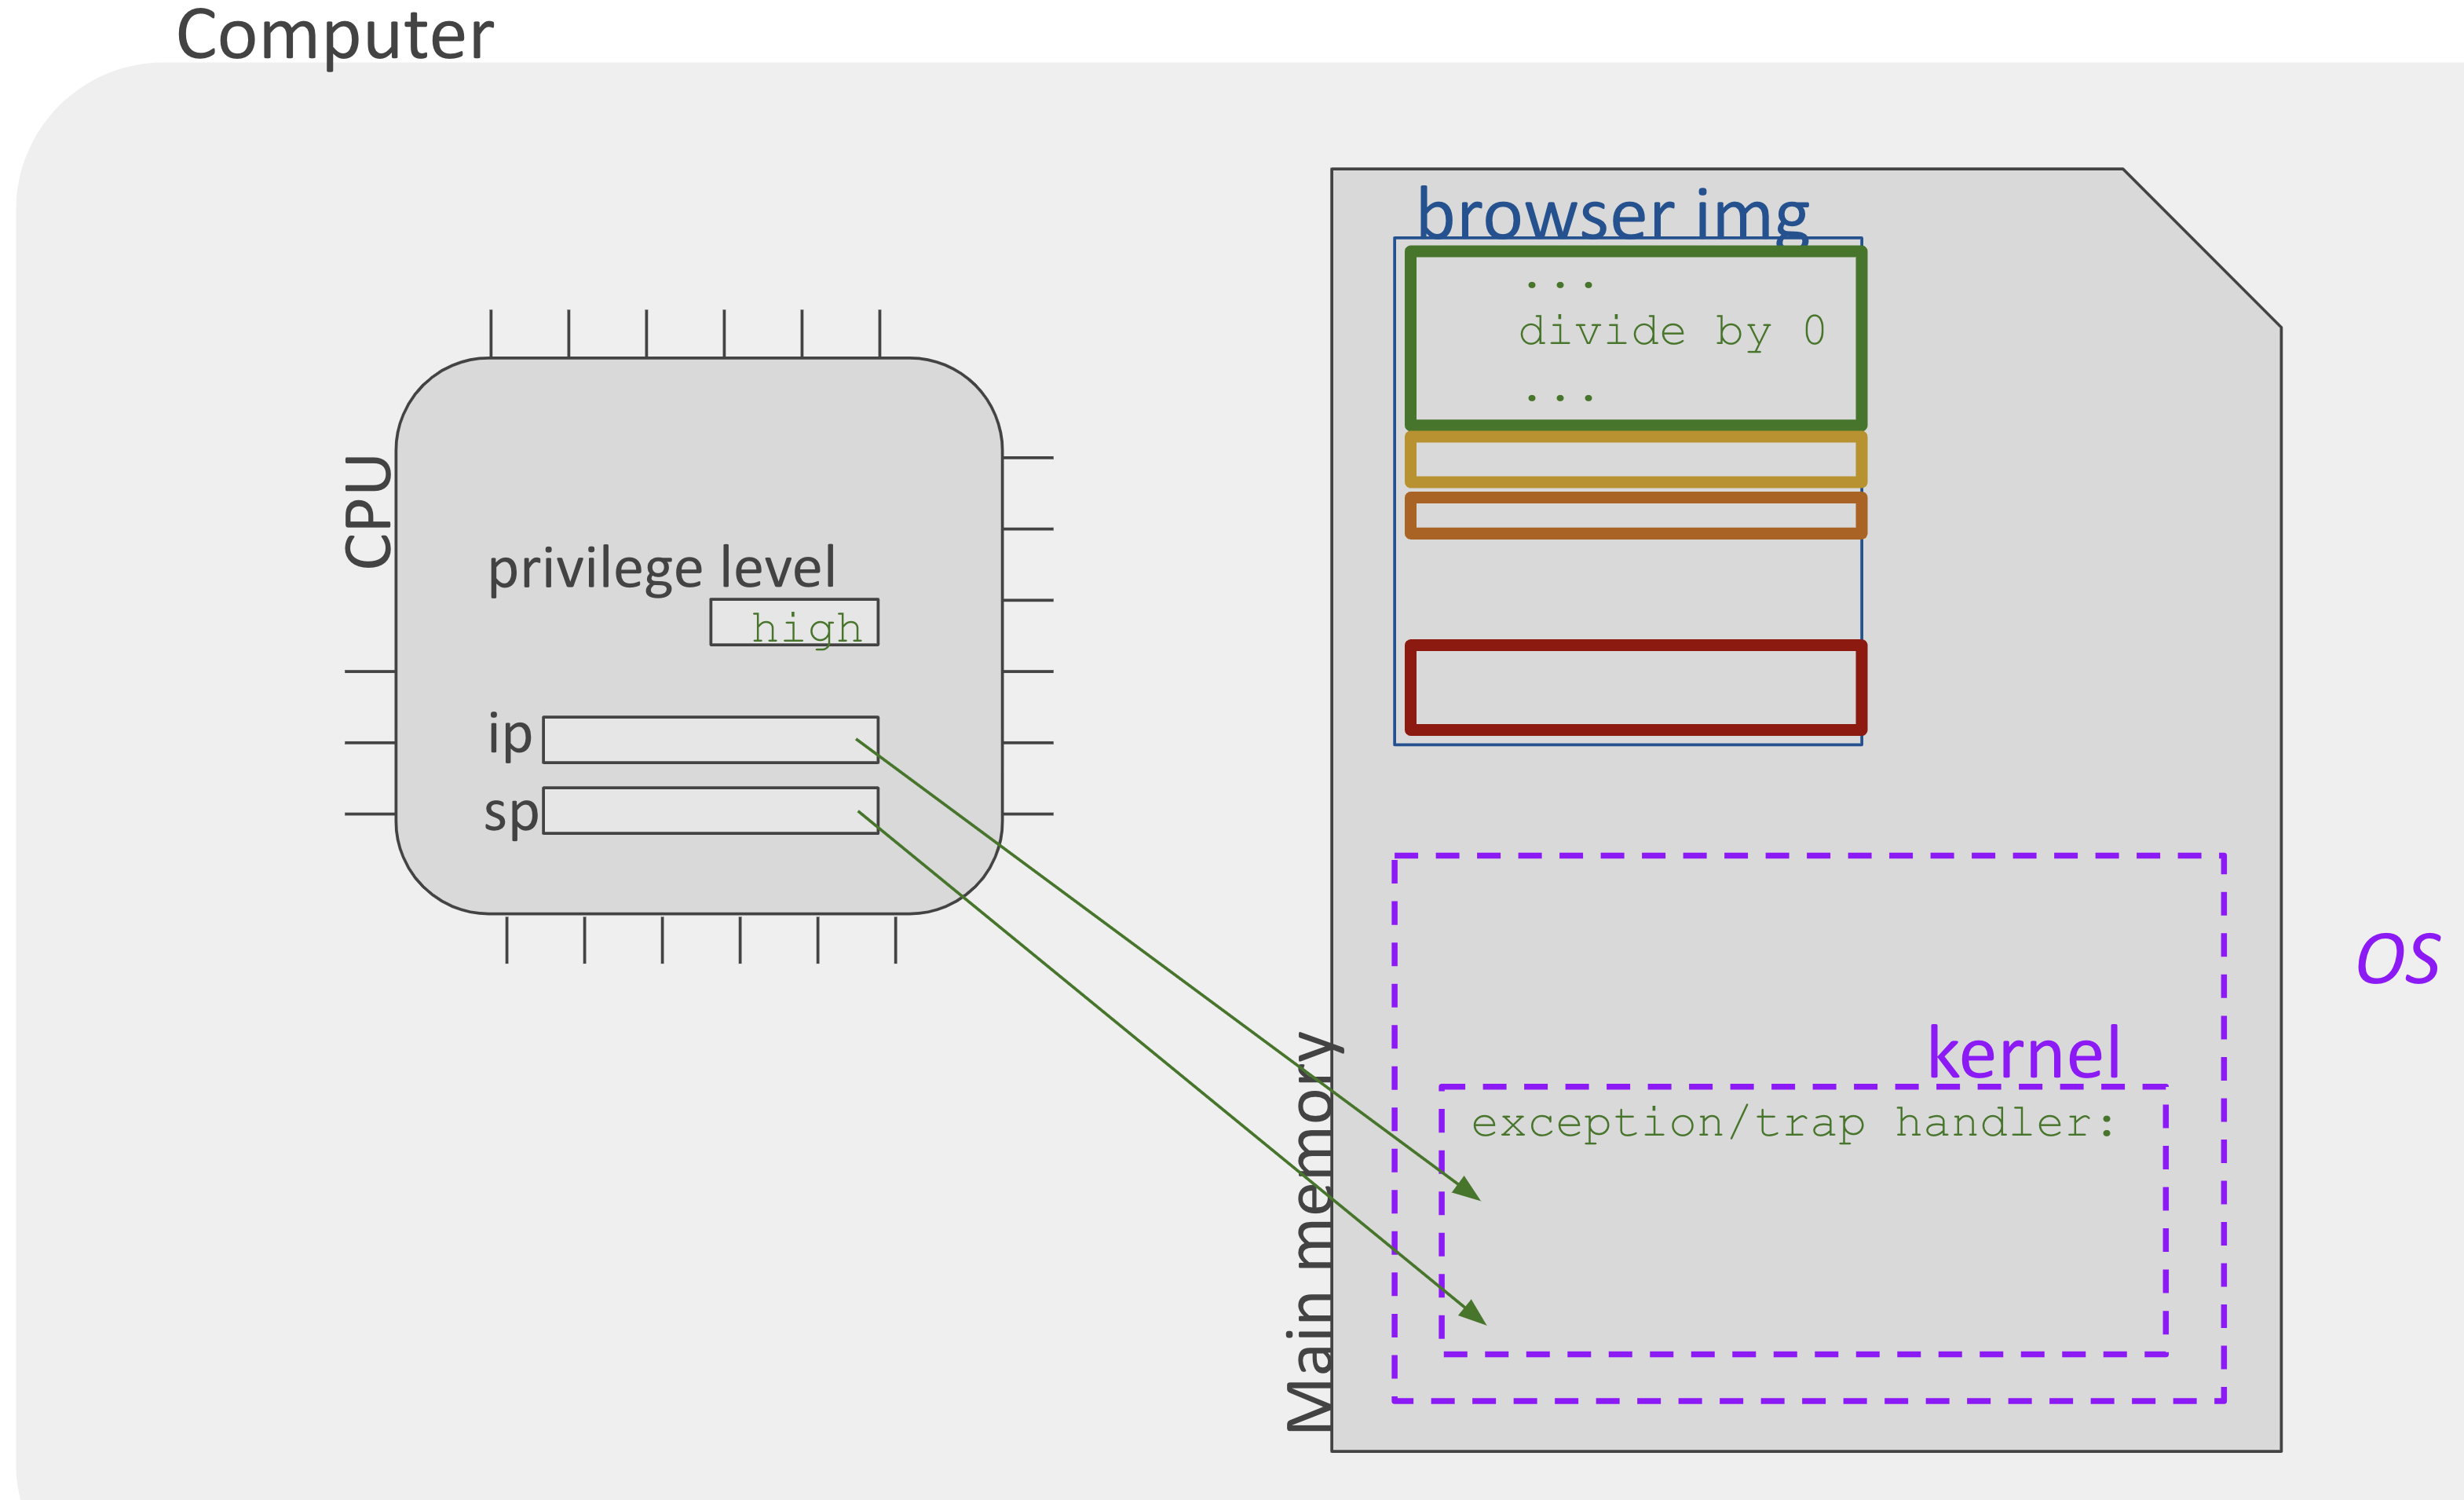
\includegraphics[width=0.95\textwidth]{chapters/L3/images/exception.png}
\end{center}
\end{minipage} 
\hfill 
\vline 
\hfill 
\begin{minipage}[htp]{0.45\textwidth}
\subsubsection*{Interrupt Handling}
Interrupts are triggered by external events and are managed by both hardware and software. The hardware raises the interrupt, and the kernel (via an interrupt handler) processes it.
\vspace{8px}
\begin{center} 
  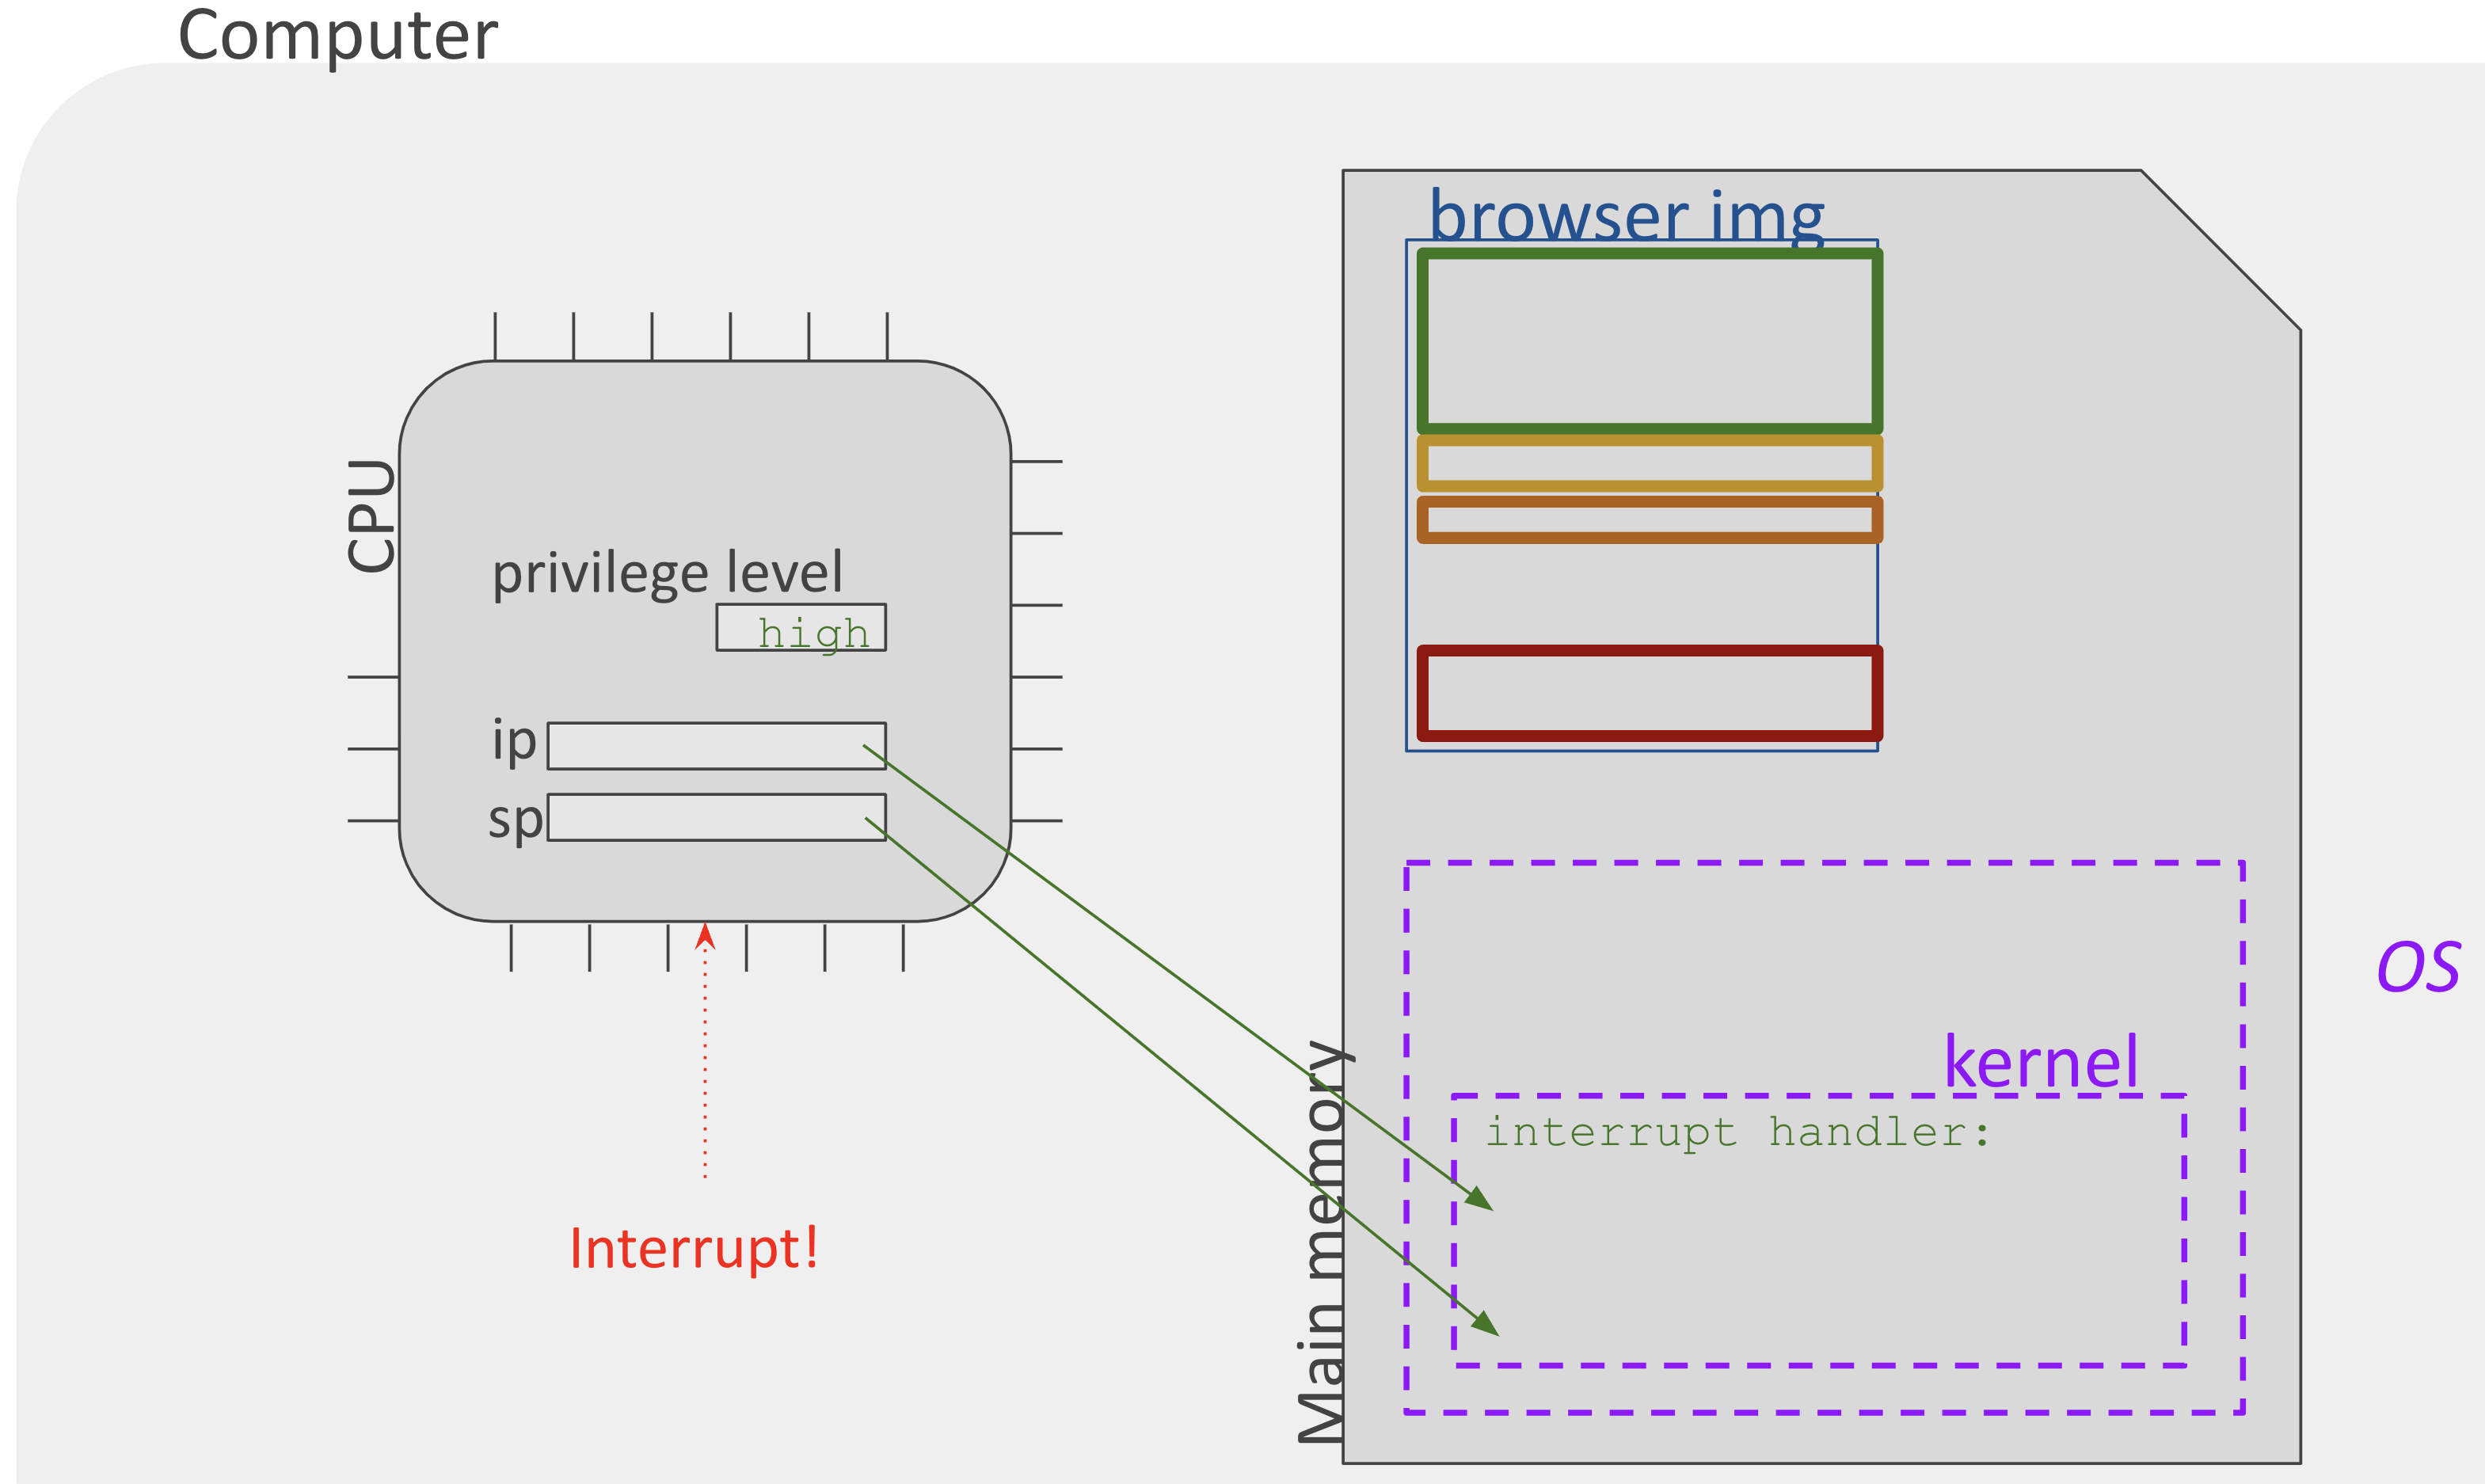
\includegraphics[width=0.95\textwidth]{chapters/L3/images/interrupt.png}
\end{center}
\end{minipage}

\subsubsection{The Timer Interrupt}
\begin{definition}[Timer Interrupt]
The timer interrupt is raised at regular intervals (typically every few milliseconds). Its handler invokes the OS scheduler to decide which process runs next, ensuring that no process monopolizes the CPU.
\end{definition}
\vspace{15px}
\newpage
\subsubsection{The OS Scheduler}
The OS scheduler manages the state transitions of processes (Running, Blocked, Ready) based on various scheduling algorithms, thereby ensuring equitable CPU access.

\begin{center}
  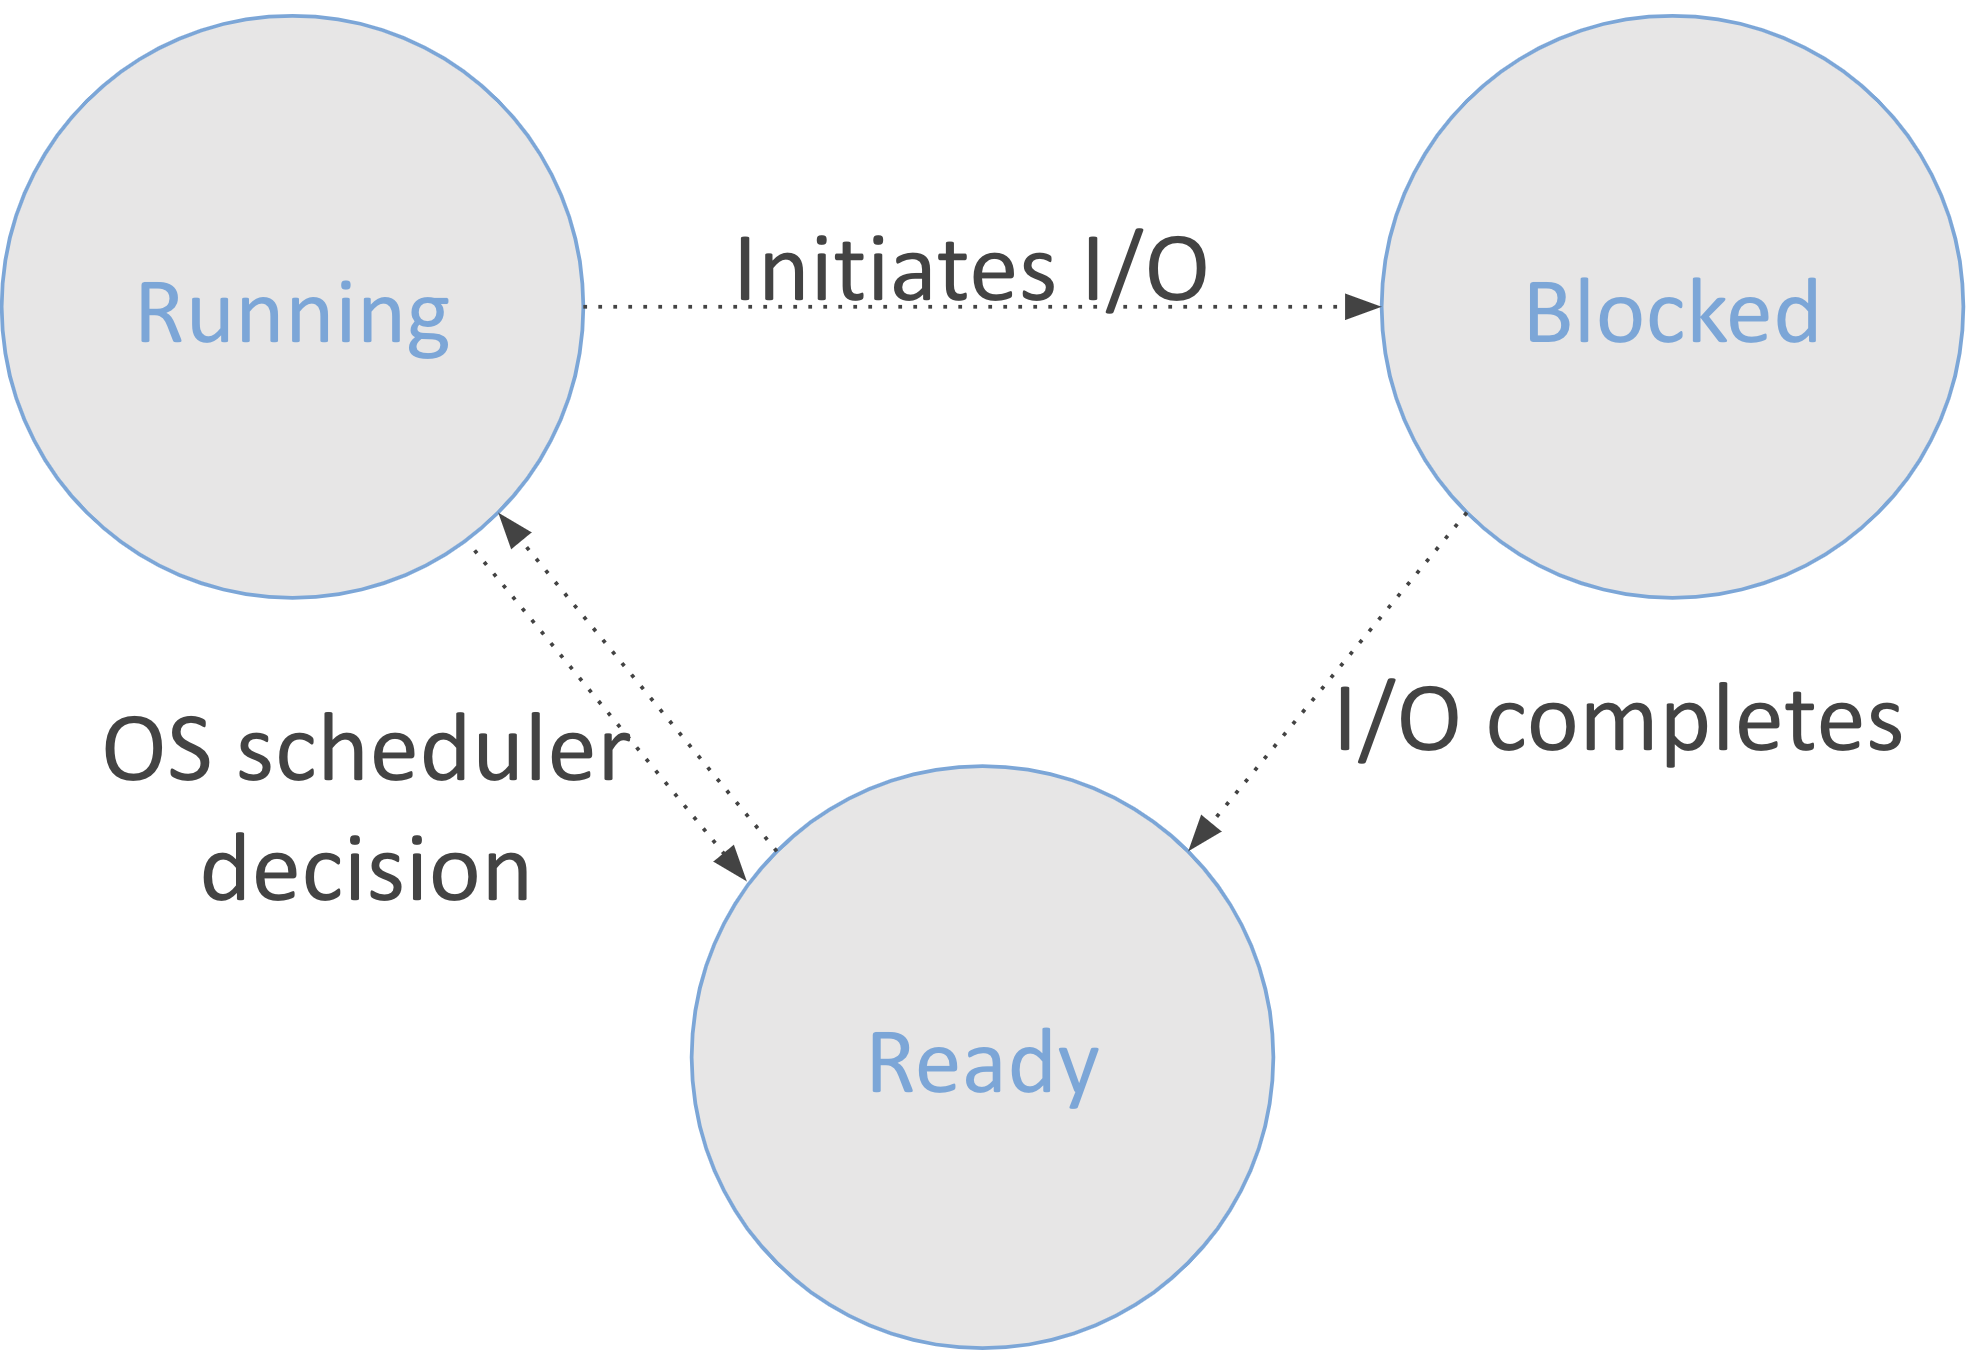
\includegraphics[width=0.45\textwidth]{chapters/L3/images/os-scheduler.png}
\end{center}

\subsection*{Summary - Limited Direct Execution}
\begin{itemize}
  \item[-] Normal threads execute in low privilege.
  \item[-] Operations requiring high privilege are performed via syscalls, exceptions, or interrupts, which invoke the kernel.
  \item[-] Timer interrupts ensure that the OS scheduler periodically gains control, maintaining fairness.
\end{itemize}

Limited direct execution is essential for safely and efficiently sharing the CPU among multiple processes.

\section{Executing Syscalls --- Process Management}

Processes are created, modified, and terminated using various syscalls. We now discuss the key syscalls involved in process management.

\subsection{Syscall Definitions}

\begin{definition}[Exit Syscall]
The \texttt{exit} syscall terminates a process. It never returns because, by the time control would return to the calling process, the process no longer exists.
\end{definition}

\begin{figure}[htp]
  \centering
  \begin{minipage}[htp]{0.45\textwidth}
\begin{cc}
_exit(0);
. 
. 
. 
. 
. 
. 
. 
. 
. 
. 
. 
\end{cc}
  \end{minipage}
  \hfill
  \vline
  \hfill
  \begin{minipage}[htp]{0.45\textwidth}
    \centering
    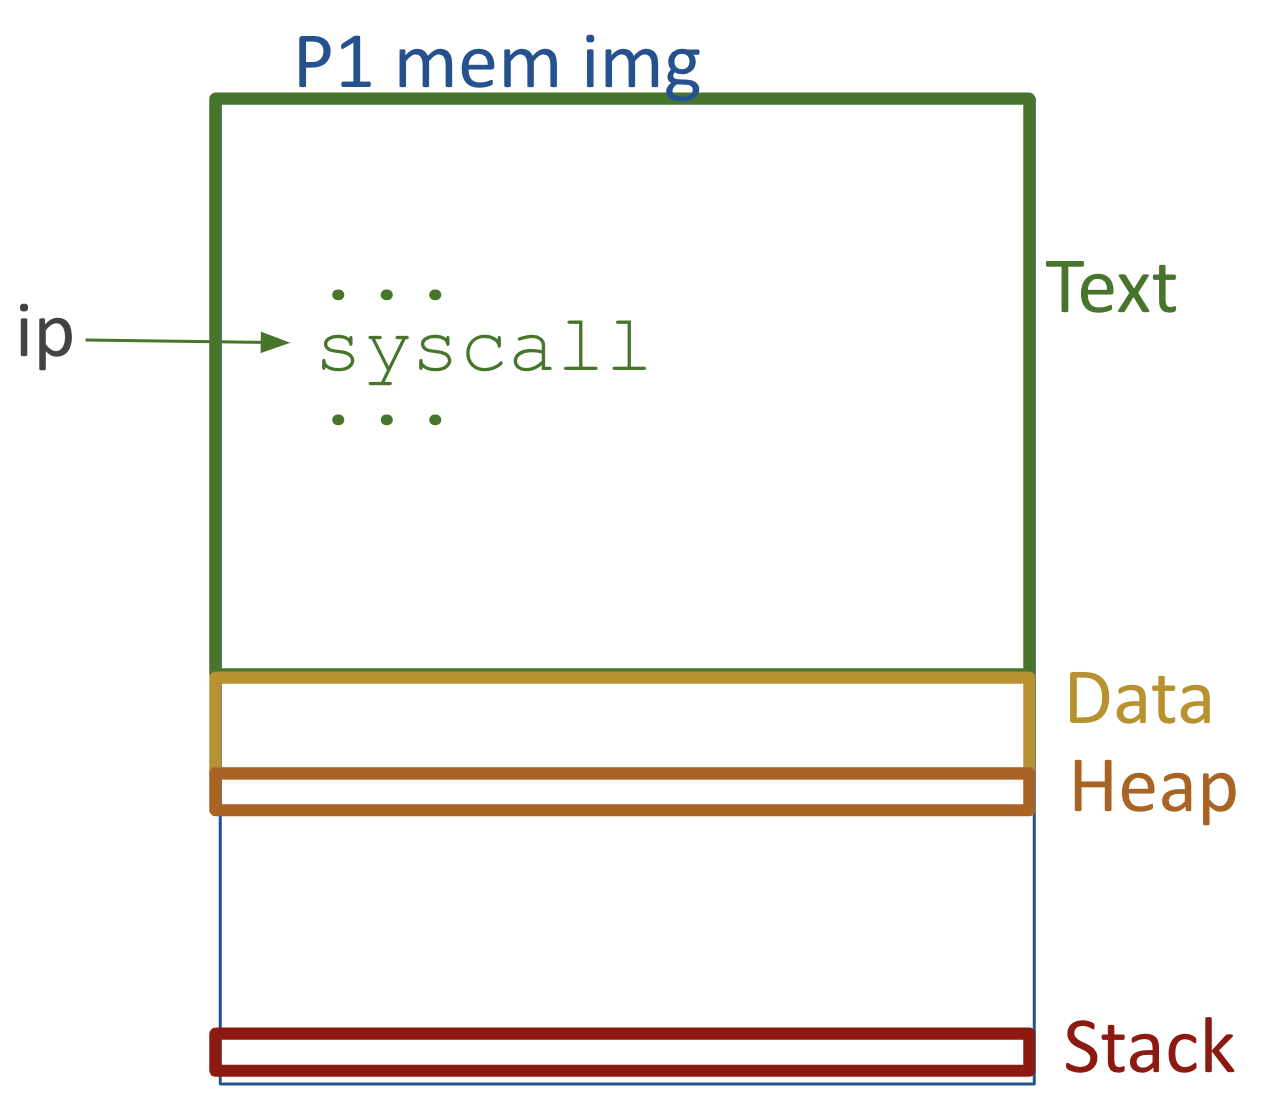
\includegraphics[width=0.8\textwidth]{chapters/L3/images/exit.png}
  \end{minipage}
  \caption{Exit Syscall: Code snippet and stack visualization.}
\end{figure}
\newpage
\begin{definition}[Exec Syscall]
The \texttt{exec} syscall replaces the current process image with a new program. It preserves the process ID and file descriptors while discarding the old program's code, data, and stack. On success, it does not return; on failure, it returns \texttt{-1}.
\end{definition}

\begin{figure}[htp]
  \centering
  \begin{minipage}[b]{0.45\textwidth}
    \begin{cc}
execvp("date", args);











    \end{cc}
  \end{minipage}
  \hfill
  \vline
  \hfill
  \begin{minipage}[b]{0.45\textwidth}
    \centering
    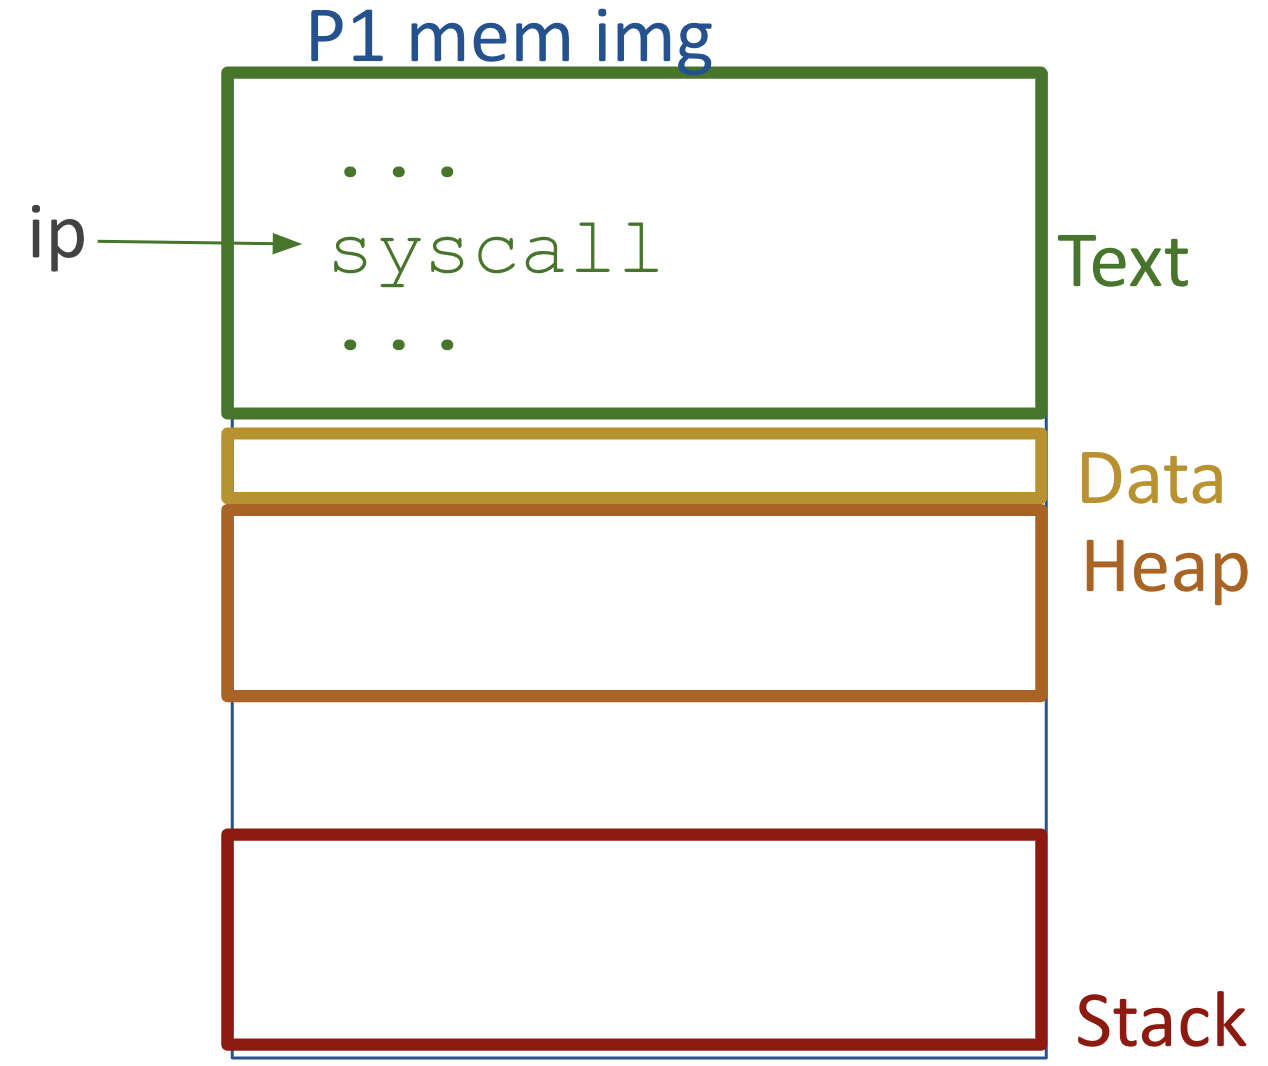
\includegraphics[width=0.8\textwidth]{chapters/L3/images/exec.png}
  \end{minipage}
  \caption{Exec Syscall: Code snippet and process image.}
\end{figure}

\begin{definition}[Fork Syscall]
The \texttt{fork} syscall creates a new child process by duplicating the calling process. Both the parent and child continue execution from the point of the fork, but in separate memory spaces. The fork returns \texttt{0} to the child and the child's process ID (PID) to the parent.
\end{definition}

\begin{figure}[htp]
  \centering
  \begin{minipage}[b]{0.45\textwidth}
    \begin{cc}
int fs = fork();
if (fs == 0) {
   // Child process code
} else {
   // Parent process code
}




    \end{cc}
  \end{minipage}
  \hfill
  \vline
  \hfill
  \begin{minipage}[b]{0.45\textwidth}
    \centering
    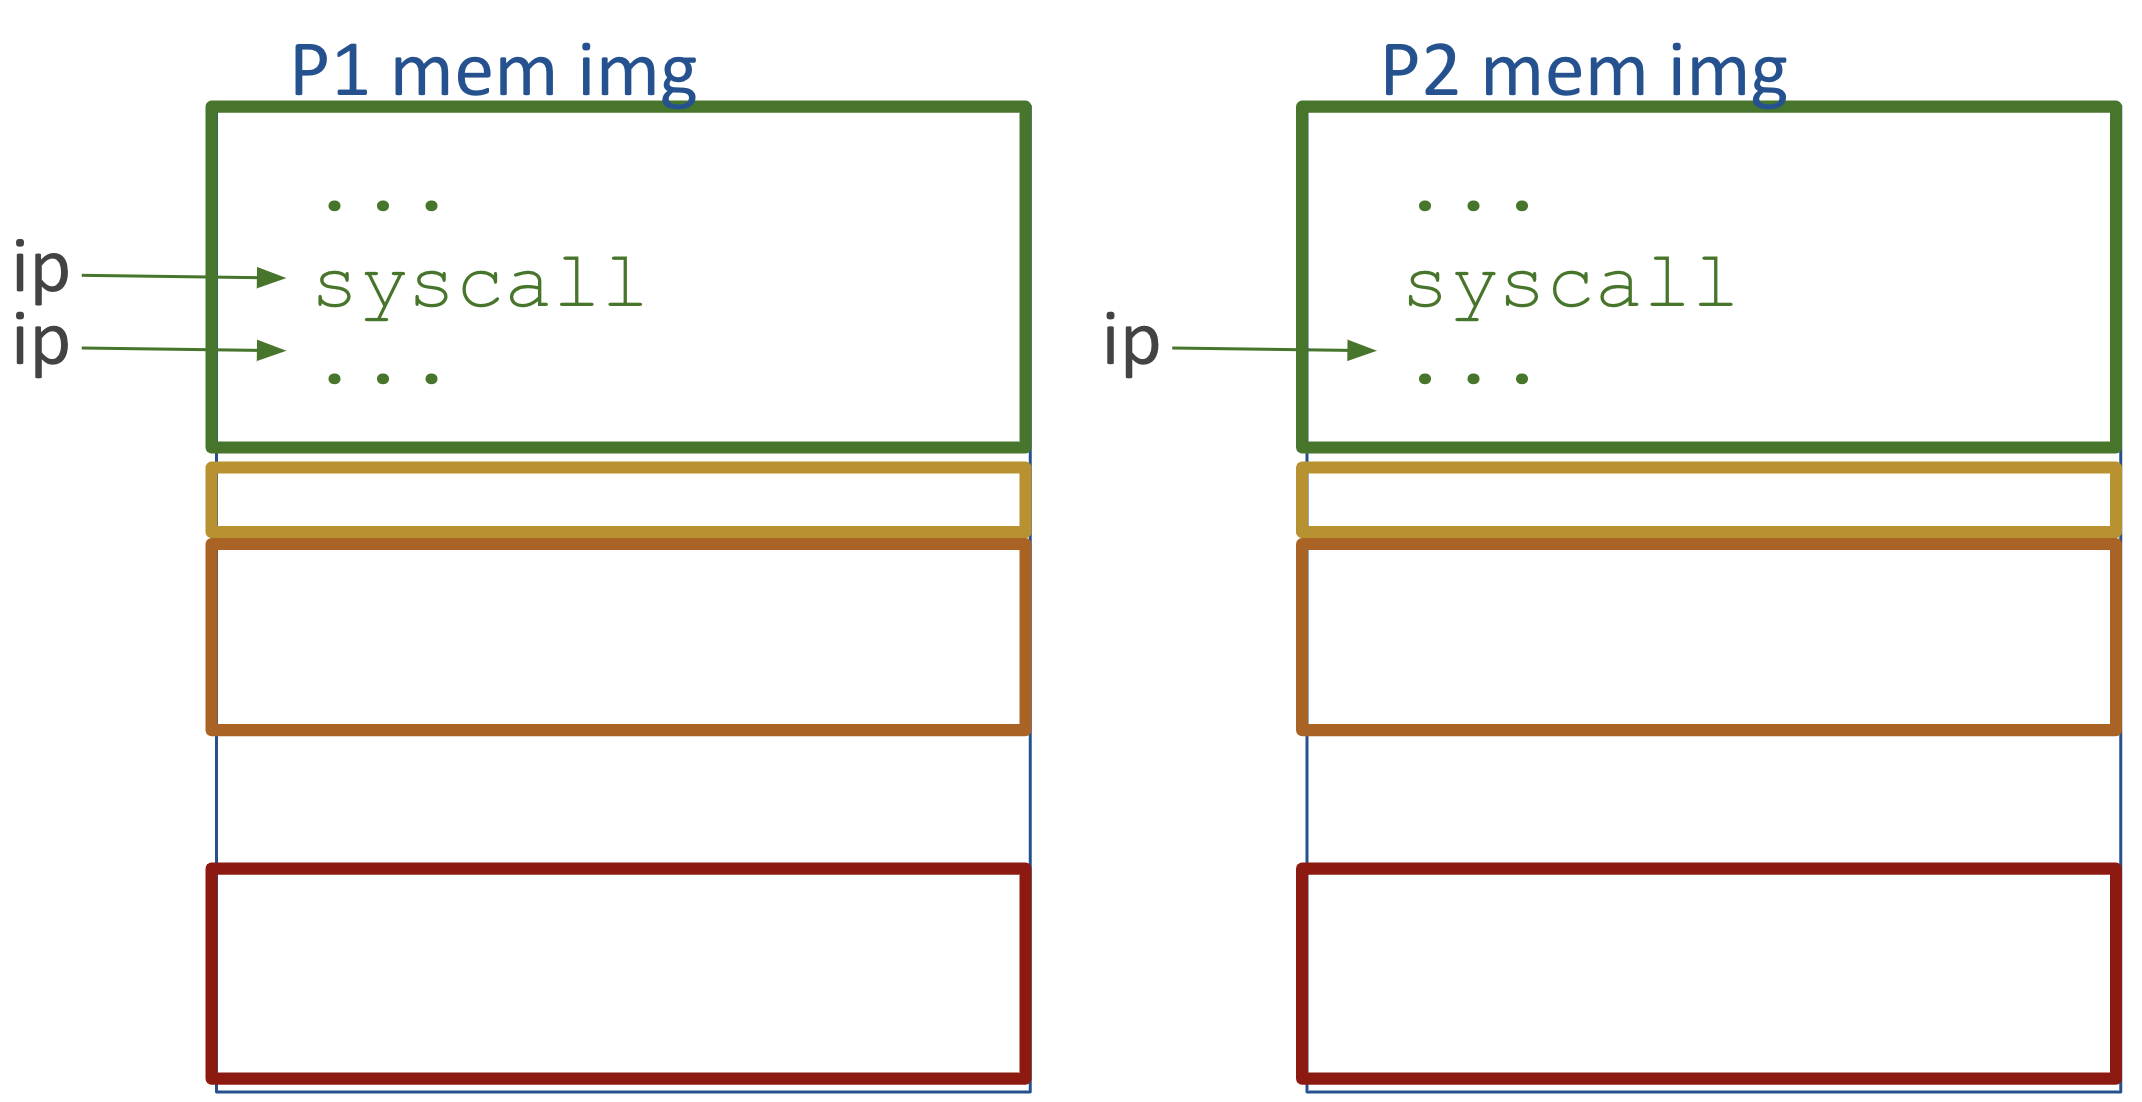
\includegraphics[width=1.25\textwidth]{chapters/L3/images/fork.png}
  \end{minipage}
  \caption{Fork Syscall: Example code and the resulting stack layout.}
\end{figure}

\begin{definition}[Wait Syscall]
The \texttt{wait} syscall allows a parent process to block until one of its child processes terminates. If no child process exists, \texttt{wait()} returns an error.
\end{definition}

\subsection{Process Creation and Cleanup}

Processes are typically created by combining the \texttt{fork} and \texttt{exec} syscalls. For example:
\begin{cc}
int fs = fork();
if (fs == 0) {
   execvp("date", args);
} else {
   wait(fs);
}
\end{cc}

When a parent process calls \texttt{wait()}, it is blocked until a child terminates, ensuring proper cleanup of child processes.
\newpage
\section{The OS Process Graph}
The OS maintains a process graph where each square represents a process and each arrow indicates the parent-child relationship. These kind of graphs are crucial for understanding process creation and hierarchy.

\begin{center}
  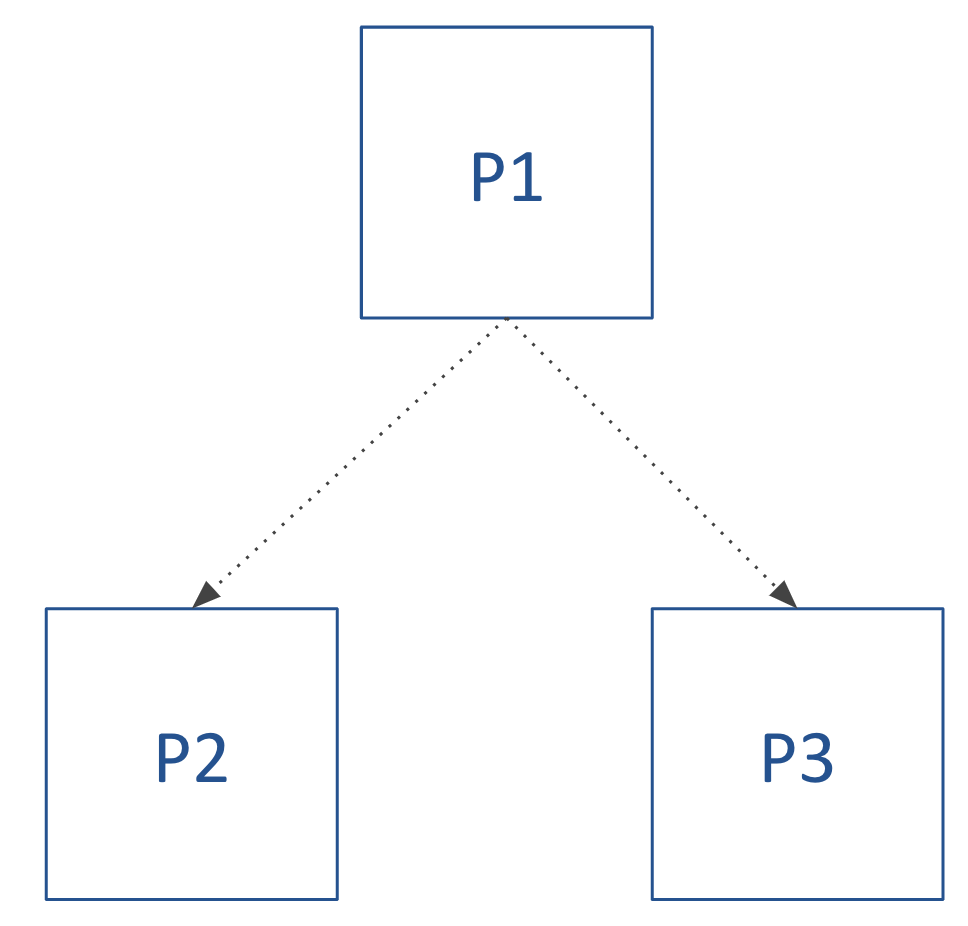
\includegraphics[width=0.25\textwidth]{chapters/L3/images/graph.png}
\end{center}

\section{Key Processes in the OS}

Some critical processes managed by the OS include:
\begin{itemize}
  \item[-] \textbf{GUI Processes:} Manage the graphical user interface.
  \item[-] \textbf{Terminal Processes:} Handle command-line interactions.
  \item[-] \textbf{Init Process:} The first process created by the kernel, responsible for starting system services.
  \item[-] \textbf{Idle Process:} Executes when no other process is runnable.
\end{itemize}

\subsection*{Conclusion - The Role of Syscalls}

Syscalls provide the interface through which processes access system resources such as storage and networks. They also facilitate self-management operations, including process creation, modification, and cleanup. Through mechanisms such as limited direct execution, exceptions, and interrupts, the OS ensures that the CPU is shared safely and efficiently among all processes.
